\documentclass[11pt,conference]{IEEEtran}

\usepackage[utf8]{inputenc}
\usepackage[T1]{fontenc}
\usepackage{amsmath,amssymb}
\usepackage{graphicx}
\usepackage{float}
\usepackage{booktabs}
\usepackage{array}
\usepackage{cite}
\usepackage{xcolor}
\usepackage{tikz}
\usetikzlibrary{arrows.meta,positioning,shapes.geometric,calc,fit,backgrounds}
\usepackage[hyphens]{url}
\usepackage[hidelinks]{hyperref}
\Urlmuskip=0mu plus 1mu
\def\UrlBreaks{\do\/\do-\do.}

\begin{document}
\title{Vision-Guided Cable Connector Insertion\\with a Kinova Gen3 Lite: Experimental Design}

\author{\IEEEauthorblockN{Sahil Gajera, Aryan Shah, Sri Satya Satwik Sirigineedi, Jay Manish Patil}
\IEEEauthorblockA{RBE 595 Final Project Report, Part 3: Experimental Design\\
Robotics Engineering, Worcester Polytechnic Institute}}

\maketitle

\begin{abstract}
This report describes how we will test the connector-insertion system on the physical robot. Four experiments cover socket localization, grasp repeatability, end-to-end pickup and insertion of audio, IEC power, and USB-A connectors, and an open-loop comparison without visual servoing. We define the test conditions, the metrics, the number of trials per condition, and the testing protocol, and we show how each experiment measures a specific target of the project.
\end{abstract}

\begin{IEEEkeywords}
experimental design, connector insertion, success rate, visual servoing, robotic assembly
\end{IEEEkeywords}

\section{Test Setup and Conditions}

\subsection{Test Bed}

All experiments run on the physical robot in the lab (Fig.~\ref{fig:setup}). The system is a Kinova Gen3 Lite with a parallel gripper and a wrist-mounted Intel RealSense D405 (848$\times$480 at 30~FPS). A fixed cradle holds the plug, and a marked board carries the 6.35~mm audio, IEC power, and USB-A sockets and a seating LED. Each connector has its own cable, which keeps the same routing in every trial.

\begin{figure}[H]
\centering
\includegraphics[width=\columnwidth]{setup_both.png}
\caption{Test bed. Left: the Gen3 Lite with the wrist D405 and the connector cradle on the table. Right: CAD of the full layout with the cradle near the base and the socket board on the vertical panel.}
\label{fig:setup}
\end{figure}

\subsection{Test Conditions}

Two factors are varied: the connector and the board pose (Table~\ref{tab:cond}, Fig.~\ref{fig:poses}). The board pose is not known to the system in advance, so shifting and turning the board tests whether the vision pipeline finds and corrects the error. The three connectors differ in clearance and keying; USB-A is the hardest. Everything else is held fixed and written in the test log: the hand-eye calibration, camera settings, the IBVS parameters, the cable routing, and the lab lighting. Calibration consistency is checked at the start of every session.

\begin{table}[H]
\caption{Test conditions.}
\label{tab:cond}
\centering
\small
\renewcommand{\arraystretch}{1.12}
\begin{tabular}{@{}p{1.75cm}p{5.9cm}@{}}
\toprule
\textbf{Factor} & \textbf{Levels}\\
\midrule
Connector & 6.35~mm audio, IEC power, USB-A\\
Board pose & P0 nominal; P1, P2: lateral shift of $\pm20$~mm; P3, P4: yaw of $\pm10^\circ$ about the insertion axis\\
\midrule
\textbf{Fixed} & Hand-eye calibration; image size 848$\times$480; IBVS desired image 200$\times$200~px square at (424, 240), gain 0.35, tolerance 5~px for 5 fresh observations, budget 800 steps and 900~s; same cable per connector\\
\bottomrule
\end{tabular}
\end{table}

\begin{figure}[H]
\centering
\resizebox{\columnwidth}{!}{%
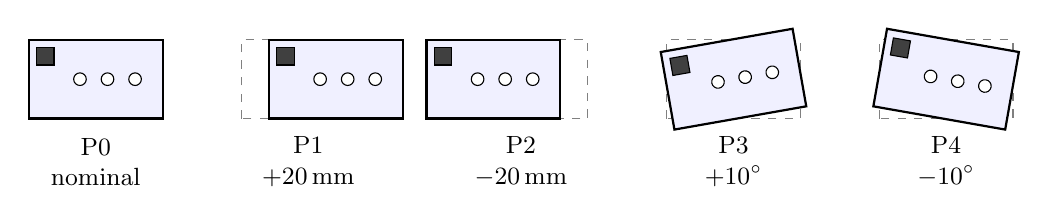
\begin{tikzpicture}[>=Stealth,font=\small]
\foreach \i/\dx/\rot/\lab in {0/0/0/{P0\\nominal},1/.35/0/{P1\\$+20$\,mm},2/-.35/0/{P2\\$-20$\,mm},3/0/10/{P3\\$+10^\circ$},4/0/-10/{P4\\$-10^\circ$}}{
 \begin{scope}[shift={(2.7*\i,0)}]
  \draw[dashed,gray] (-.85,-.5) rectangle (.85,.5);
  \begin{scope}[shift={(\dx,0)},rotate=\rot]
   \draw[thick,fill=blue!6] (-.85,-.5) rectangle (.85,.5);
   \draw[fill=black!75] (-.75,.18) rectangle (-.53,.4);
   \draw[fill=white] (-.2,0) circle (.08);
   \draw[fill=white] (.15,0) circle (.08);
   \draw[fill=white] (.5,0) circle (.08);
  \end{scope}
  \node[align=center] at (0,-1.05) {\lab};
 \end{scope}}
\end{tikzpicture}}
\caption{Board-pose conditions seen from the front. The dashed outline is the nominal pose, the dark square is the marker, and the three circles are the sockets. Shifts are in the board plane, and yaw is about the insertion axis.}
\label{fig:poses}
\end{figure}

\begin{table*}[!t]
\caption{Performance metrics, targets, and the experiment that measures each.}
\label{tab:metrics}
\centering
\small
\renewcommand{\arraystretch}{1.15}
\begin{tabular}{@{}p{3.3cm}p{8.6cm}p{3.6cm}p{1.2cm}@{}}
\toprule
\textbf{Metric} & \textbf{Definition} & \textbf{Target} & \textbf{Exp.}\\
\midrule
Grasp success $G$ & Plugs still held after a 10~cm lift and a 3~s hold without visible slip, divided by all grasp attempts & $\geq$ 95\% & E2, E3\\
Insertion success $S$ & $S=n_{\mathrm{seated}}/N$, where a trial is seated within two attempts and verified independently; reported with a 95\% Wilson interval~\cite{wilson1927} & Audio $\geq$ 90\%, IEC $\geq$ 80\%, USB-A $\geq$ 70\% & E3, E4\\
First-attempt success $S_1$ & Fraction of trials seated on the first attempt, with no retry & Reported & E3, E4\\
Localization error & Position error $e_p=\lVert\hat{\mathbf p}-\mathbf p_{\mathrm{ref}}\rVert$ and yaw error $e_\psi=|\hat\psi-\psi_{\mathrm{ref}}|$ against the taught reference; mean and 95th percentile & Mean $e_p<2$\,mm and $e_\psi<3^\circ$ & E1\\
Alignment error & Final RMS corner error of the IBVS features in pixels, and the number of steps to converge & $\leq$ 5\,px for 5 fresh observations & E3\\
Cycle time $T$ & Time from the start of the pick motion to verified seating, over successful trials; mean and standard deviation. Total time including scans is also logged & Mean $<60$\,s & E3\\
Failure causes & Share of failed trials per cause (perception, grasp, alignment, insertion, verification) & Reported & E2, E3, E4\\
\bottomrule
\end{tabular}
\end{table*}

\subsection{Status}

One supervised USB-A pickup and a 55~mm commanded extraction were completed on the real robot, and the IBVS stage converged to about 5~px. Repeated trials have not yet been run, so no success rate exists yet. The experiments below produce it. Figures~\ref{fig:overlay} and~\ref{fig:stages} show the pilot pickup that the E2 and E3 pick stage repeats. It is a single supervised demonstration, so it shows that the stage runs and not how reliable it is.

\begin{figure}[H]
\centering
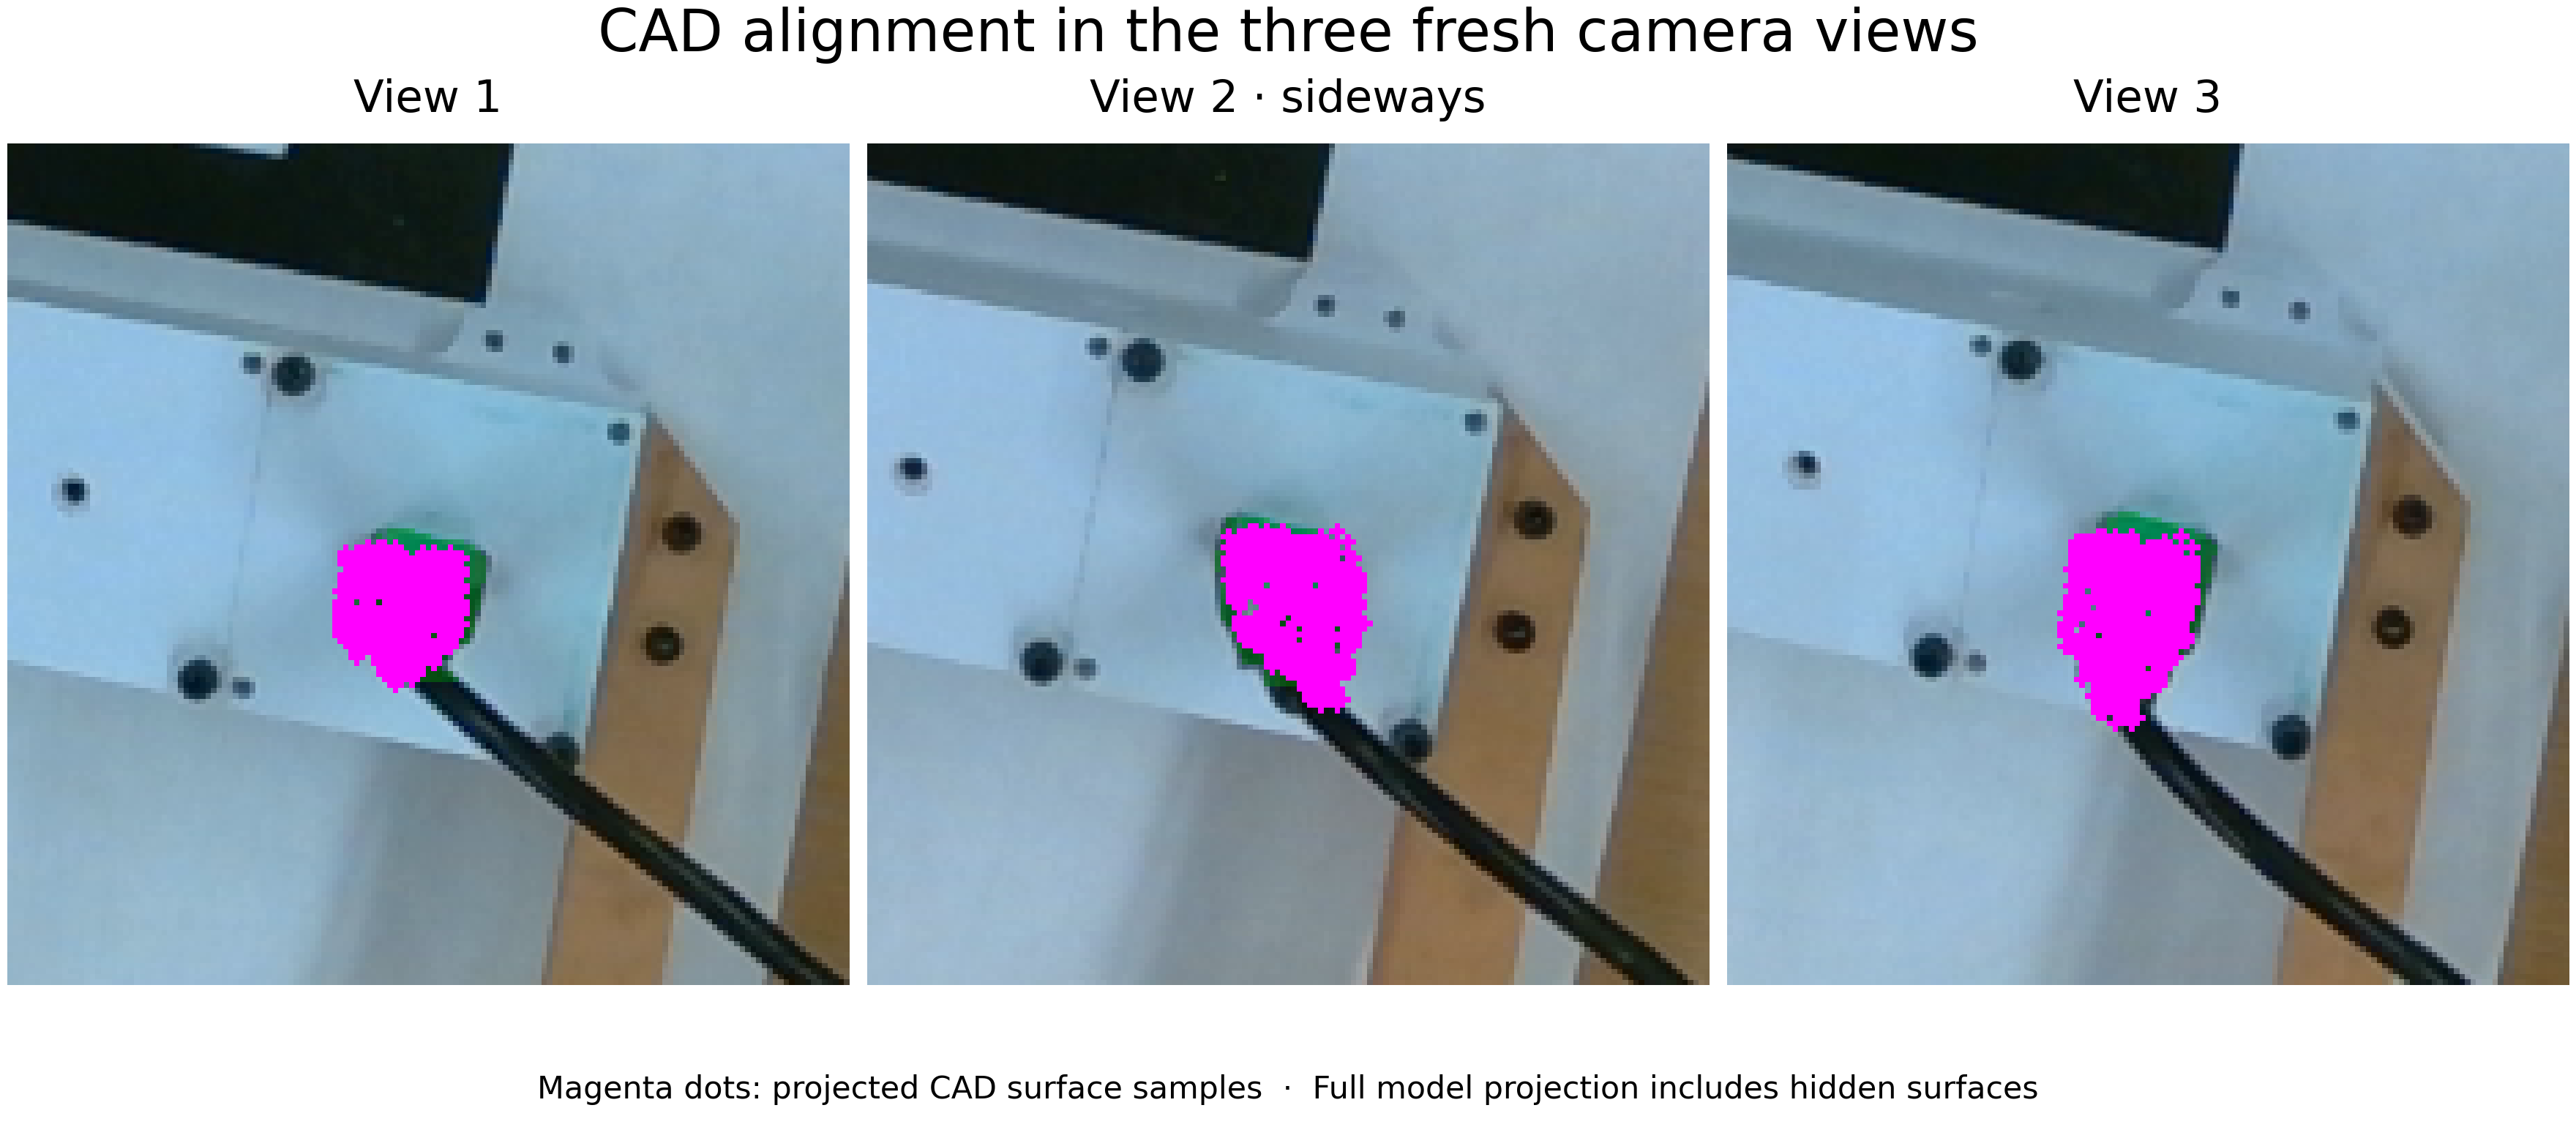
\includegraphics[width=\columnwidth]{04_camera_cad_overlays.png}
\caption{Pilot USB-A pickup: the fitted CAD surface (magenta) projected into the three fresh wrist-camera views. Held-out median surface residuals were 1.15, 1.25 and 0.61~mm. These are depth-to-CAD residuals, not absolute grasp accuracy.}
\label{fig:overlay}
\end{figure}

\begin{figure}[H]
\centering
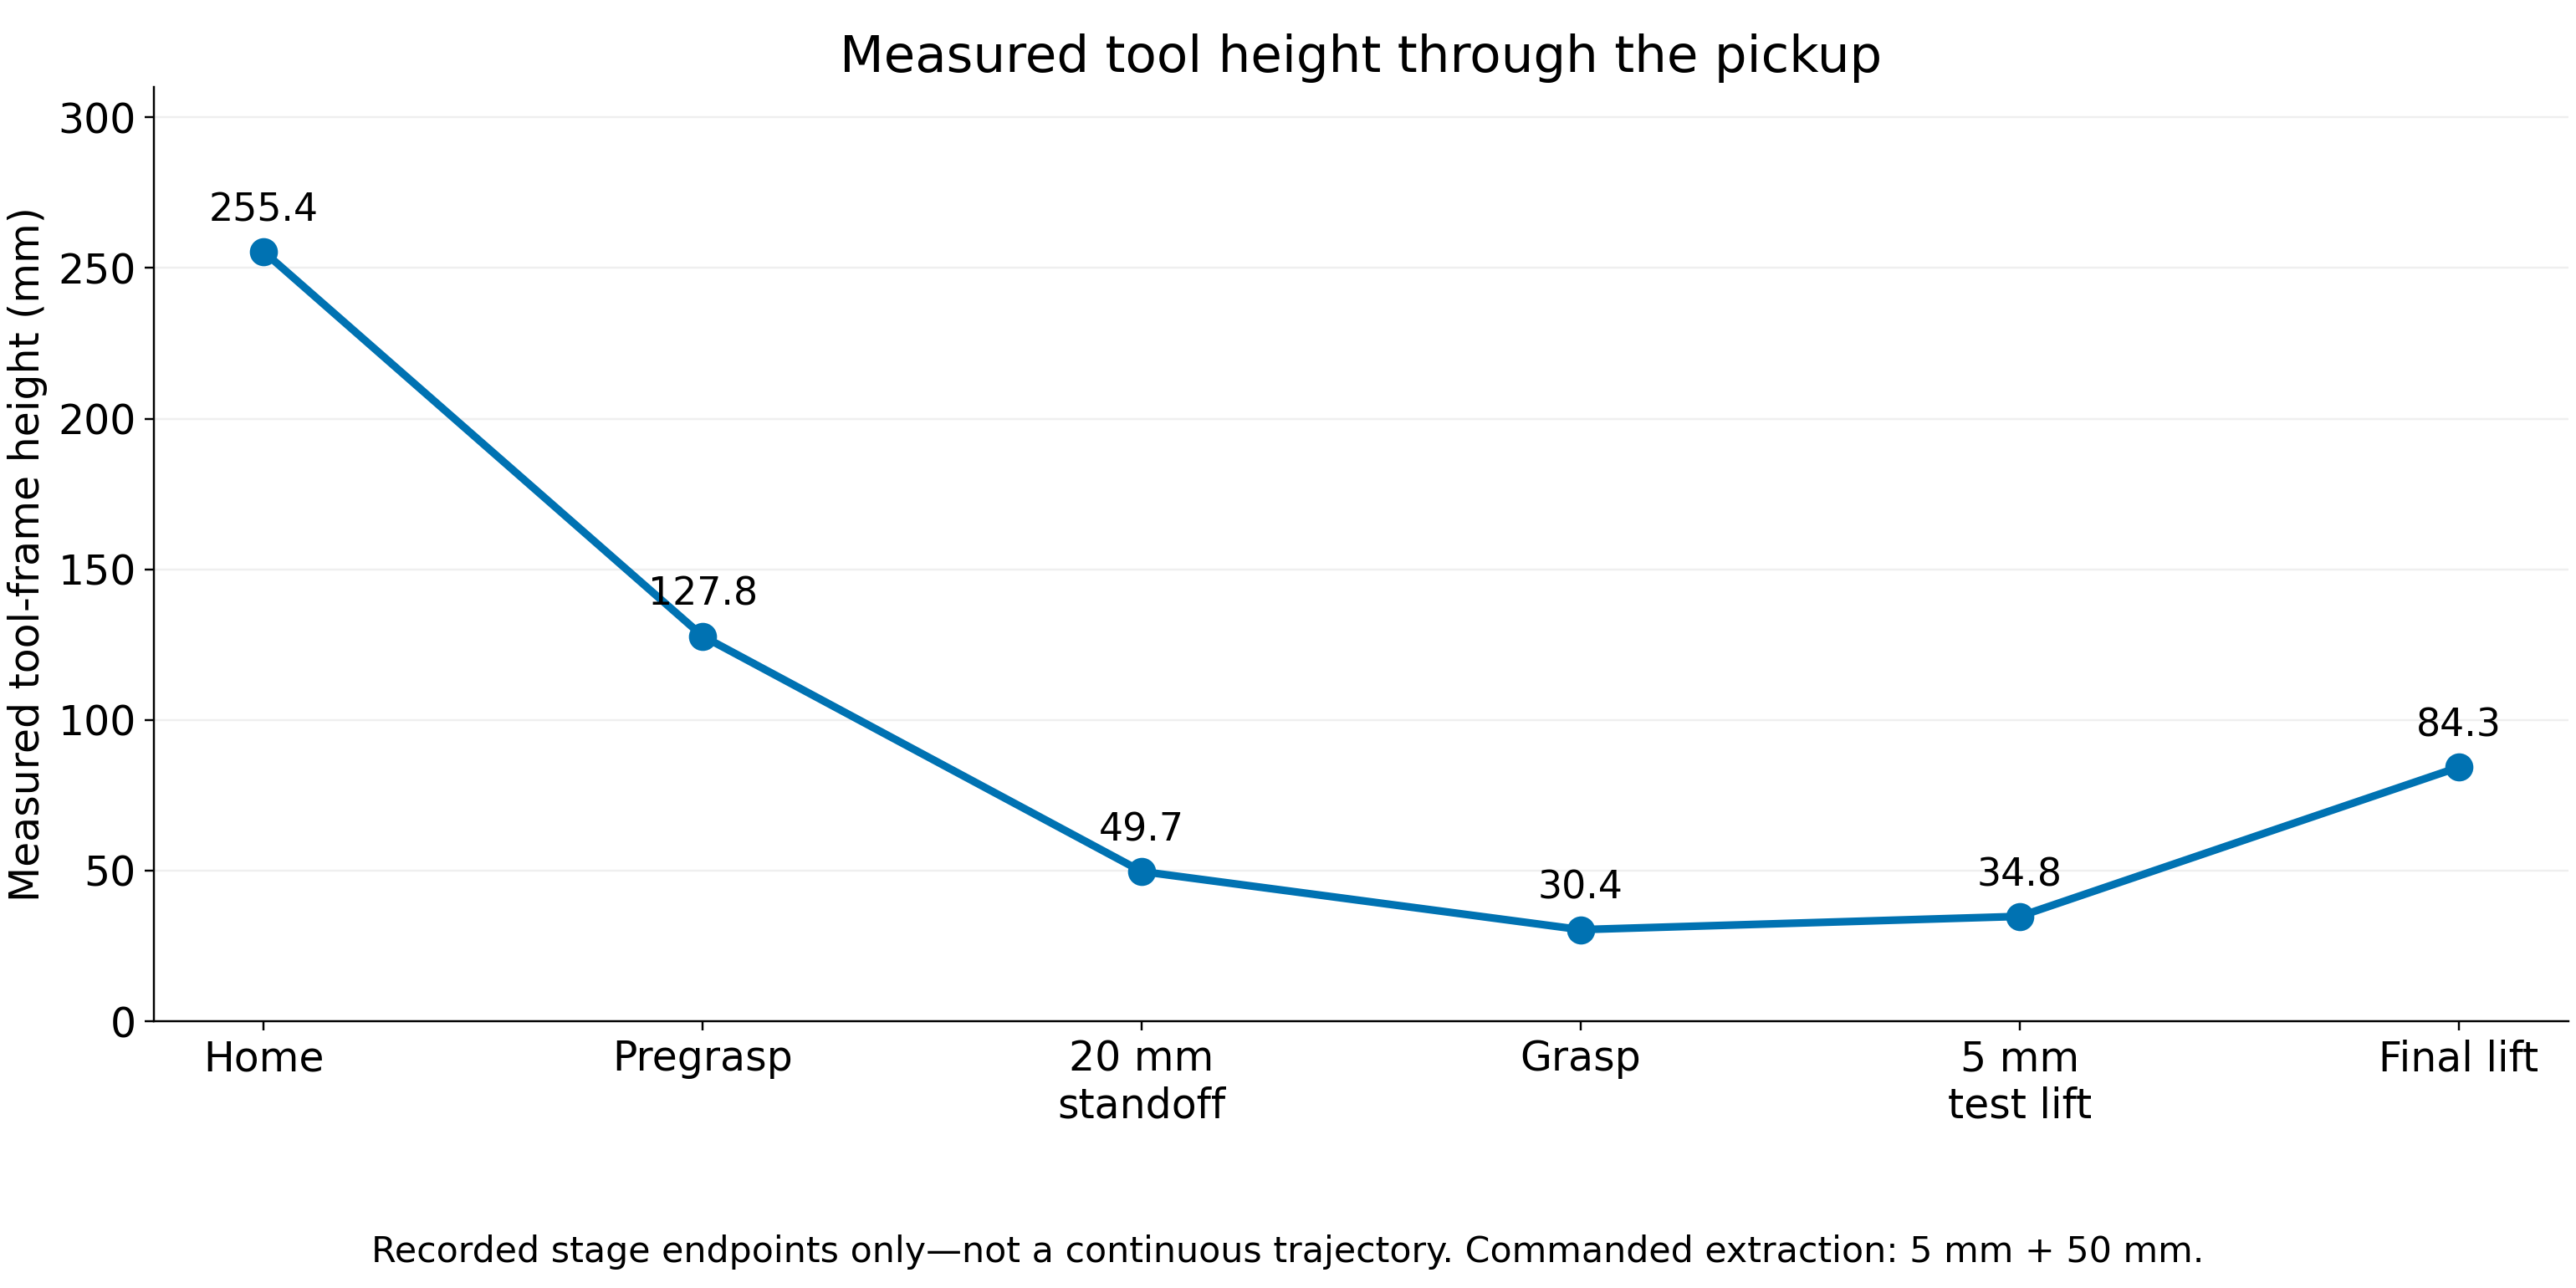
\includegraphics[width=\columnwidth]{06_measured_pickup_stages.png}
\caption{Pilot pickup: measured tool-frame height at the recorded stage endpoints (not a continuous trajectory). The commanded extraction was 5~mm plus 50~mm. Holding was confirmed by the operator, since encoder feedback alone does not verify it. E2 adds an independent slip check after a 10~cm lift.}
\label{fig:stages}
\end{figure}

\section{Experimental Procedure}

We run four experiments. E1 to E3 are required, and E4 is run if time permits.


\textbf{E1: Socket localization (no insertion).} The board is set to each pose in Table~\ref{tab:cond}, the arm scans it, and the estimated socket pose is recorded. The reference is a taught pose: the gripper tip is jogged to the socket entrance and its forward-kinematics pose is read. The taught pose is repeated three times per board pose to measure its own spread, and the CAD offsets of P1 to P4 are checked with a ruler.

\textbf{E2: Grasp repeatability.} For each connector, the plug is placed in the cradle and the robot runs the pick stage only: three views, CAD fit, pregrasp at a 100~mm standoff, staged approach, gripper closure, extraction, and a 10~cm lift with a 3~s hold. The operator then returns the plug to the cradle.

\textbf{E3: End-to-end pickup and insertion.} The full pipeline runs for each connector and board pose, following the trial procedure in Fig.~\ref{fig:procedure}. This is the main experiment, and its metrics are in Table~\ref{tab:metrics}.

\textbf{E4: Open-loop comparison.} E3 is repeated without the IBVS stage. The arm goes from the standoff pose computed from the marker pose directly to the insertion. This shows what visual servoing adds. It uses the same schedule seed, plug, cable and calibration as E3, so the only change is the missing IBVS stage. Because E3 has 8 nominal trials and E4 has 2, E4 is compared with the full E3 set and with a matched subset of E3 (2 trials per pose, chosen by the fixed seed).

\textbf{Localization error definition (E1).} Each estimated socket entrance pose $(\hat{\mathbf p},\hat\psi)$ is expressed in the robot base frame. The reference $(\mathbf p_{\mathrm{ref}},\psi_{\mathrm{ref}})$ is the mean of the three taught readings for that board pose, and their standard deviation is reported as the noise floor of the reference. An error is read as meaningful only if it exceeds this spread.

\textbf{Retry rule.} After a first failed insertion (stall, depth short of $d_{\mathrm{seat}}$, or LED off), the arm retreats to the standoff pose, rescans the board, reruns IBVS, and applies a small lateral offset toward the residual error before the second push. The offset size is fixed during the pilot runs and frozen with the other parameters. No other parameter changes between attempts. Any hand intervention during a trial ends it as a failure.

\begin{figure}[H]
\centering
\resizebox{\columnwidth}{!}{%
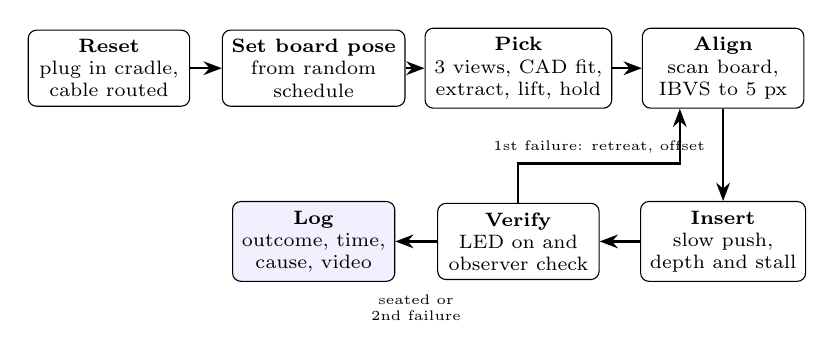
\begin{tikzpicture}[>=Stealth,font=\scriptsize,
 bx/.style={draw,rounded corners=3pt,align=center,minimum height=.95cm,minimum width=2.05cm,fill=white},
 lab/.style={fill=white,inner sep=1pt,font=\tiny},
 arr/.style={->,thick}]
\node[bx] (rs) at (0,0) {\textbf{Reset}\\plug in cradle,\\cable routed};
\node[bx] (pp) at (2.6,0) {\textbf{Set board pose}\\from random\\schedule};
\node[bx] (pk) at (5.2,0) {\textbf{Pick}\\3 views, CAD fit,\\extract, lift, hold};
\node[bx] (al) at (7.8,0) {\textbf{Align}\\scan board,\\IBVS to 5 px};
\node[bx] (in) at (7.8,-2.2) {\textbf{Insert}\\slow push,\\depth and stall};
\node[bx] (vf) at (5.2,-2.2) {\textbf{Verify}\\LED on and\\observer check};
\node[bx,fill=blue!6] (lg) at (2.6,-2.2) {\textbf{Log}\\outcome, time,\\cause, video};
\draw[arr] (rs) -- (pp);
\draw[arr] (pp) -- (pk);
\draw[arr] (pk) -- (al);
\draw[arr] (al) -- (in);
\draw[arr] (in) -- (vf);
\draw[arr] (vf) -- (lg);
\node[font=\tiny,align=center,anchor=north] at (3.9,-2.75) {seated or\\2nd failure};
\coordinate (r1) at ($(vf.north)+(0,.5)$);
\coordinate (r2) at ($(al.south)+(-.55,-.0)$);
\draw[arr] (vf.north) -- (r1) -| (r2);
\node[font=\tiny,above] at ($(r1)!.5!(r1 -| r2)$) {1st failure: retreat, offset};
\end{tikzpicture}}
\caption{One trial. A first failed insertion retreats and aligns again; a second failed attempt, or a verified seating, ends the trial and the result is logged.}
\label{fig:procedure}
\end{figure}

\textbf{Trial procedure.} A trial follows Fig.~\ref{fig:procedure}. The operator resets the plug and cable and sets the scheduled board pose. The robot then picks the plug, scans the board, aligns with IBVS, and inserts. A trial allows at most two insertion attempts in total. Seating is judged independently of the controller: the trial counts as seated only if the socket LED is on and the observer confirms the plug is flush with the socket face. The robot's own depth reading is logged but does not decide the result.

\section{Performance Metrics}

Table~\ref{tab:metrics} lists the metrics and their targets. All rates are computed per connector unless stated otherwise. Failures are assigned to one cause from the logs and video: \emph{perception} (bad CAD fit or socket pose), \emph{grasp} (no stable hold), \emph{alignment} (IBVS does not converge within its budget), \emph{insertion} (stall or hard stop), or \emph{verification} (the robot's belief and the independent check disagree).

\textbf{Hypotheses.} We state the expected outcomes before running, so the results can refute them.
\begin{itemize}
\item H1: Visual alignment keeps the localization error below 2~mm and $3^\circ$ (E1), so seating success at P1 to P4 is not far below P0 (E3).
\item H2: Success falls in the order audio, IEC, USB-A, because clearance shrinks and keying tightens in that order.
\item H3: Without IBVS (E4), success drops mainly at the displaced poses P1 to P4. At P0 the open-loop result may be close to E3, so a small difference there does not count against the method.
\end{itemize}


\section{Number of Trials and Testing Protocol}

\subsection{Trial Counts}

Table~\ref{tab:trials} gives the plan. The end-to-end experiment E3 uses 20 trials per connector: 8 at the nominal pose P0 and 3 at each of P1 to P4. This gives a nominal-pose result and also covers the displaced poses. E2 uses 20 grasps per connector, E1 uses 4 scans at each of the 5 board poses, and E4 uses 10 trials per connector with 2 at each pose. That is 170 runs in total.

Twenty trials give a usable but wide estimate. When the observed rate equals a target exactly (18, 16, or 14 successes of 20), the 95\% Wilson interval is still about $\pm14$ to 19 points wide (Fig.~\ref{fig:ci}). Ten trials would make it another 11 to 12 points wider in total. Prior work uses from 12 trials per method~\cite{peng2020comparison} and 20 trials~\cite{she2021cable} up to 100 to 150 trials per condition~\cite{haugaard2020,lian2021}, and the NIST task-board protocol notes that few trials limit how far a rate can be trusted~\cite{kimble2020}. We therefore report every rate with its interval and do not claim a target is proven by one run of 20 trials.

\begin{table}[H]
\caption{Trial plan.}
\label{tab:trials}
\centering
\small
\renewcommand{\arraystretch}{1.12}
\begin{tabular}{@{}p{.8cm}p{2.9cm}p{2.3cm}p{1.2cm}@{}}
\toprule
\textbf{Exp.} & \textbf{Conditions} & \textbf{Per connector} & \textbf{Total}\\
\midrule
E1 & 5 board poses & 4 per pose & 20\\
E2 & Cradle only & 20 grasps & 60\\
E3 & P0 $\times$ 8, P1--P4 $\times$ 3 & 20 trials & 60\\
E4 & P0--P4 $\times$ 2, no IBVS & 10 trials & 30\\
\bottomrule
\end{tabular}
\end{table}

\begin{figure}[H]
\centering
\resizebox{\columnwidth}{!}{%
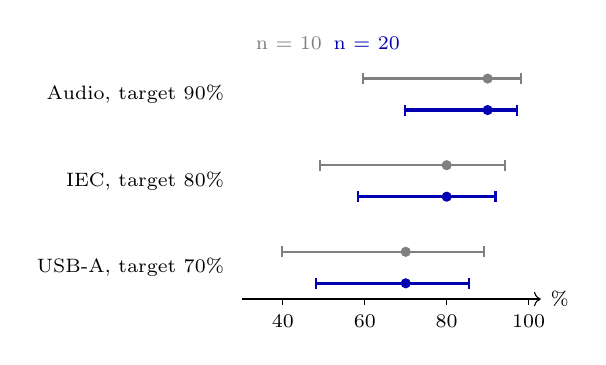
\begin{tikzpicture}[font=\scriptsize,x=.052cm,y=1cm]
\draw[->] (30,0) -- (103,0) node[right]{\%};
\foreach \v in {40,60,80,100}{\draw (\v,0)--(\v,-.08) node[below]{\v};}
\foreach \y/\name/\a/\b/\c/\d/\p/\q in {2.6/{Audio, target 90\%}/59.6/98.2/69.9/97.2/90/90,
                                      1.5/{IEC, target 80\%}/49.0/94.3/58.4/91.9/80/80,
                                      .4/{USB-A, target 70\%}/39.7/89.2/48.1/85.5/70/70}{
 \node[anchor=east,align=right] at (28,\y) {\name};
 \draw[gray,thick] (\a,\y+.2)--(\b,\y+.2);
 \draw[gray,thick] (\a,\y+.13)--(\a,\y+.27) (\b,\y+.13)--(\b,\y+.27);
 \node[circle,fill=gray,inner sep=1.3pt] at (\p,\y+.2) {};
 \draw[blue!70!black,very thick] (\c,\y-.2)--(\d,\y-.2);
 \draw[blue!70!black,thick] (\c,\y-.27)--(\c,\y-.13) (\d,\y-.27)--(\d,\y-.13);
 \node[circle,fill=blue!70!black,inner sep=1.3pt] at (\q,\y-.2) {};}
\node[gray,anchor=west] at (31,3.25) {n = 10};
\node[blue!70!black,anchor=west] at (50,3.25) {n = 20};
\end{tikzpicture}}
\caption{95\% Wilson intervals when the observed rate exactly equals each target, for 10 and 20 trials per connector.}
\label{fig:ci}
\end{figure}

\subsection{Protocol}

\begin{itemize}
\item \emph{Freeze before testing.} All parameters are set in pilot runs, which are not counted. They are frozen before E1 to E4 start, so the results do not include tuning.
\item \emph{Order.} Board poses follow a random schedule with a fixed seed. Connectors are run in blocks, and the order of blocks changes between sessions so that drift does not favor one connector.
\item \emph{Session start.} Home the arm, check the hand-eye calibration on the calibration marker, and record the time and lighting.
\item \emph{Reset.} After every trial the plug is returned to the cradle, the cable is routed the same way, and the board is set to the next pose.
\item \emph{Discarded trials.} Only faults unrelated to the method (a driver crash or a lost camera frame stream) are discarded and repeated. They are counted and listed in the report. Any collision or unsafe motion triggers the emergency stop and is counted as a failure.
\item \emph{Logging.} Each trial stores the connector, board pose, schedule index, saved RGB-D views and CAD-fit metrics, the estimated socket pose, final IBVS error and steps, stage times, insertion depth against $d_{\mathrm{seat}}$, stall events, attempts, outcome, failure cause, and video.
\item \emph{Statistics.} Rates use 95\% Wilson intervals, times use mean and standard deviation, and errors use mean and 95th percentile.
\end{itemize}

\subsection{Pilot Runs and Parameter Freezing}
Before data collection we run uncounted pilot trials at P0 for each connector to set the standoff distance, IBVS gain, push speed, stall threshold and retry offset. A parameter set is frozen only after 3 consecutive pilot trials finish without a software fault. The frozen values, the code commit and the calibration file are written to the header of the test log. If a parameter must change after freezing, every counted trial of the affected experiment is rerun.

\subsection{Safety and Abort Rules}
The operator stays at the emergency stop for every trial, and insertion uses the slow velocity-controlled push. A trial is aborted and counted as a failure if (i) the end effector hits anything other than the target socket, (ii) the plug is dropped, or (iii) the 900~s budget runs out. After any abort the arm is homed and the calibration check is repeated before the next trial. Three consecutive aborts end the session, and the cause is found before testing resumes.

\subsection{Analysis Plan}
Success is also tabulated per board pose as a descriptive breakdown. With 3 to 8 trials per cell it is too small for inference. The E3 and E4 difference in $S$ and $S_1$ is tested with Fisher's exact test and reported as a difference in proportions. A target counts as \emph{met} when the point estimate reaches it, and as \emph{supported} only when the lower Wilson bound is above 50\%. Times are reported as mean, standard deviation and median, because retries can skew cycle time. Per-trial logs and all videos are archived so that any result can be re-scored.

\section{Connection to Target Performance}

The task goal is to pick the plug, align with the matching socket, and seat it fully, recording success, time, and failed attempts. Table~\ref{tab:link} ties each target to the experiment that measures it and to its decision rule.

\begin{table}[H]
\caption{How each experiment tests a target.}
\label{tab:link}
\centering
\small
\renewcommand{\arraystretch}{1.12}
\begin{tabular}{@{}p{2.2cm}p{1.3cm}p{4.1cm}@{}}
\toprule
\textbf{Target goal} & \textbf{Exp.} & \textbf{Decision rule}\\
\midrule
Reliable pickup & E2, E3 & $G\geq95\%$ over all grasps\\
Accurate socket pose & E1 & Mean $e_p<2$\,mm, $e_\psi<3^\circ$\\
Seat all three connectors & E3 & $S\geq$ 90, 80, 70\% (18, 16, 14 of 20)\\
Visual correction helps & E3, E4 & $S$ and $S_1$ of E3 higher than E4\\
Fast enough & E3 & Mean $T<60$\,s\\
Understand failures & E2--E4 & Failure causes reported\\
\bottomrule
\end{tabular}
\end{table}

These experiments measure success because the end-to-end trial in E3 is the task itself: the same pipeline, the real sockets, and a seating check that does not depend on the robot's own estimate. E1 and E2 isolate the two stages that feed it, so a failure in E3 can be traced to localization or grasping. The board poses in E3 create the pose uncertainty the system is designed to handle, and E4 shows whether the visual-servoing stage is the reason for success. Hypotheses H1 to H3 map to the rows of Table~\ref{tab:link}: H1 to localization and seating at displaced poses, H2 to the per-connector targets, and H3 to the E3 and E4 comparison. The target rates match whole-number successes in 20 trials, so the pass rule is easy to apply.

The experiments have limits. They use one board, one cable per connector, and one lab lighting condition, and they do not measure contact force because the arm has no wrist force sensor. The 20-trial intervals are wide, so the results show whether the system is near each target and not whether it exceeds it by a small margin.

% ---- OPTIONAL: add a simulation comparison only if the simulation baseline is kept in the report ----
% \textbf{E5: Simulation-to-real comparison.} The same conditions and success definitions are run in simulation, and the success rates and times are compared with E3.

\bibliographystyle{IEEEtran}
\bibliography{references}

\end{document}
